\section{Snap!}
\label{solution SNAP}
Ce travail part d'un environnent de programmation existant : \gls{snap}. Ce projet a pour but de fournir une interface et un environnement supportant la programmation par \glspl{bloc}. Cependant, ce projet ne s'inscrit pas dans le cadre d'un apprentissage scolaire ou guidé. Il a donc fallu l'adapter. Cette partie explique les différentes adaptations apportées au projet d'origine et pourquoi elles sont nécessaires pour remplir les objectifs.\\

Dans les adaptations opérées, sont retenus : une simplification de l'interface, une différenciation des \glspl{role} entre le professeur et le public cible, le masquage des \glspl{script}, une amélioration de la traduction en français et la sauvegarde sur les serveurs du projet courant.

\subsection{L'interface}
\label{interface}
Comme expliqué précédemment, \gls{snap} n'a pas une vocation didactique de groupe et a un public cible plus large. Il a des menus pour des fonctionnalités de gestion de l'ordonnanceur, des options d'affichage, des paramètres d'éditions, etc. Certaines de ces fonctionnalités sont trop complexes et/ou peuvent distraire inutilement le public visé par \gls{rsnap}.

Un nettoyage en profondeur de l'interface de \gls{snap} a été opéré afin de laisser uniquement les menus utiles. Toutefois, ils n'ont pas été effacés, mais masqués afin qu'il puissent être utilisés par les professeurs, comme il est discuté dans les \glspl{role} \ref{role}.\\

Une autre adaptation de l'interface est l'ajout d'un menu pour les interactions avec la plateforme web. Ce menu contient des boutons tels que :
\begin{itemize}
  \item "sauvegarder sur le serveur", pour enregistrer le travail de l'étudiant sur la plateforme ;
  \item "description", pour permet de retrouver le résumé introductif de la \gls{mission} ;
  \item "retour à la liste des missions", pour sauvegarder le travail puis renvoyer vers la page listant les \glspl{mission} sur le site web.
\end{itemize}

\subsection{Les rôles}
\label{role}
Afin de fournir une interface épurée pour les étudiants comme expliqués dans la section \ref{interface}, il est nécessaire d'enlever des parties non pertinentes de l'interface de \gls{snap}. Toutefois, ces options inutiles aux étudiants peuvent l'être pour les professeurs et également pour une \gls{mission} en "mode ouvert". Il est donc utile d'avoir une interface modulaire suivant son utilisation. \\

Pour différencier les utilisations de l'interface, la notion de \glspl{role} a été ajoutée. Deux \glspl{role} sont définis : étudiant et professeur. Ainsi, quand un élève ouvrent un projet, \gls{snap} est lancé avec le rôle étudiant, ce qui permet de ne pas afficher les options superflues. Quand un professeur souhaite modifier une \gls{mission} ou en créer une nouvelle, \gls{rsnap} lance \gls{snap} avec le rôle professeur ce qui donne accès aux fonctions avancées de \gls{snap}.\\

Ces \glspl{role} permettent également la gestion du masquage de \glspl{script}. Il est intéressant qu'un professeur puisse masquer des \glspl{bloc}, sans que les étudiants ne puissent les réafficher.

\subsection{Masquer les scripts}
Pour la création des \glspl{mission}, il a été nécessaire de cacher des \glspl{bloc} aux élèves. Par exemple, la partie de vérification du code de l'élève ou encore le code de l'environnement de la \gls{mission} ne doivent pas leur apparaître.

Une possibilité de cacher des \glspl{bloc} existait déjà dans la zone des \glspl{bloc} sources (voir la figure \ref{fig:cacher}) de l'interface. Cette fonctionnalité est étendue pour pouvoir également cacher des \glspl{bloc} ou des \glspl{script} dans la partie d'édition (voir la figure \ref{fig:snap interface}).

Il a donc fallu ajouter cette information dans la sauvegarde du projet. Ceci a été réalisé grâce à la balise \texttt{hidden} dans le XML.\\


Cette fonctionnalité étant intéressante pour le projet original, elle a été proposée dans une \texttt{\gls{pull}}. Les responsables de \gls{snap} ont marqué leur intérêt pour cette fonctionnalité qui est toujours en cours d'étude.
\begin{figure}
  \begin{center}
    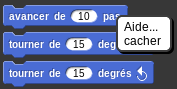
\includegraphics[scale=0.5]{content/7-solution/2-snap/images/cacher}
    \caption{Option pour cacher la définition d'un bloc}
    \label{fig:cacher}
  \end{center}
\end{figure}

\subsection{Traduction}
Ce travail se différencie des autres initiatives similaires introduites dans la section \ref{travail associe} par son caractère francophone. L'application était déjà traduite partiellement en français, mais une large majorité des traductions était incomplète, inexistante ou erronée. Il a donc fallu en améliorer la traduction. La traduction de l'application est différente pour la partie interface et la partie fournissant les aides.

Des aides étaient déjà disponibles en anglais. La possibilité de les avoir dans d'autres langues a été développée pour ce travail. De plus, des aides en français étaient déjà existantes dans le projet SCRATCH \cite{scratch-translation}. C'est donc elles qui ont été utilisées pour \gls{snap}.

L'ensemble de ces aménagements a été proposé au projet original. Il a été accepté et il sera intégré après quelques modifications du serveur utilisé par \gls{snap}.

\subsection{Sauvegarde sur le serveur}
Comme il est nécessaire d'interfacer l'environnement de programmation avec un site web, l'implémentation de certaines fonctionnalités d'import-export spécifiques à \gls{rsnap} a été réalisée.

Il est nécessaire de disposer d'un fichier XML pour sauvegarder les \glspl{mission} sur le serveur. Les fonctions existantes ont été adaptées pour permettre d'avoir ce fichier et de pouvoir l'envoyer au serveur.
